
\documentclass[a4paper,12pt]{article}
\title{projectreport}
\usepackage[top=1in, bottom=1in, left=1in, right=1in]{geometry}
\usepackage{epsfig}
\usepackage[nottoc]{tocbibind}
\usepackage{float}
\usepackage{multicol}
\usepackage{graphicx}
\usepackage{titlesec}
\usepackage{lipsum}
\usepackage{caption}
\usepackage{subcaption}
\usepackage{booktabs}
%\usepackage[dvips]{graphics}
\usepackage{sectsty}
\usepackage{chngcntr}
\usepackage[hidelinks]{hyperref}
\usepackage{algorithmic}
\usepackage{algorithm2e}
 \usepackage{booktabs}
%\usepackage[dvips]{graphics}
\sectionfont{\centering}
%\usepackage{helvet}
%\renewcommand{\familydefault}{\sfdefault}
%\usepackage{titlesec}
%\setkomafont{section}{\normalfont\huge\sffamily\bfseries\color{blue}}
%\renewcommand{\rmdefault}{phv} % Arial
%\renewcommand{\sfdefault}{phv} % Arial
\renewcommand{\abstractname}{\large Abstract}
\counterwithin{figure}{section}
\newcommand*{\myfont}{\fontfamily{Arial}\selectfont}
\renewcommand{\baselinestretch}{1.5}
\bibliographystyle{elsarticle-num}

\begin{document}

\pagenumbering{gobble}
\thispagestyle{empty}
\begin{center}
\textit{Major Project Report on} \\
\vspace{2 mm}
\Large{\textsc{ Remote Operating System Image Management }}   % Your major Project Title

\vspace{7 mm}
\large{\textbf{                  % Group members name
Gaurav U D ( 16IT113 )  
\\Abhilash V ( 16IT201 )   
\\Rahul A R ( 16IT239 ) 
}}
\\
\vspace{4 mm}
Under the Guidance of\\
\textbf{Dr. Jaidhar C D}\\         % Name of your guide
Department of Information Technology, NITK Surathkal\\
\vspace{4 mm}
\textit{Date of Submission: 18/02/2020}
\\
\vspace{4 mm}
in partial fulfillment for the award of the degree
\\
%\vspace{3 mm}

of

\textbf{Bachelor of Technology}

In

\textbf{Information Technology}

At
\vspace{4 mm}
    
        
\includegraphics[width=1.5in,height=1.5in]
        {nitk.jpg}
 
\textbf{Department of Information Technology}

\textbf{National Institute of Technology Karnataka, Surathkal}

\textbf{February 2020}
\end{center}

%%%%%%%%%%%%%%%%%%%%%%%%%%%% Page 2 %%%%%%%%%%%%%%%%%%%%%%%%%%%%%%%%%%%%%%


\begin{center}
\textbf{\large{Department of Information Technology, NITK Surathkal}} \\

\textbf{\large{Major Project - II}} \\
\textbf{\large{Progress Report (February 2020)}} \\
\noindent\rule{12cm}{0.4pt}
\end{center}


\noindent
\textbf{Course Code :} IT 499 \\
\textbf{Course Title:} Major Project - II \\
\textbf{Project Title:} \emph{Remote OS Image cloning and  deployment management}   % update project title

\subsubsection*{Project Group:}
\begin{tabular}{lcl}
\hline                         % Update name of students here 
Name of the Student & Register No. & Signature with Date             \\
\hline
Gaurav U D            &16IT113        &                            \\\\
Abhilash V            &16IT201        &                            \\\\
Rahul A R            &16IT239        &                            \\\\
\hline
\end{tabular} 

\vspace{5 em}

Place:

Date:\hfill \textit{(Name and Signature of Major Project Guide)}


%%%%%%%%%%%%%%%%%%%%%%%%%%% Page 3 %%%%%%%%%%%%%%%%%%%%%%%%%%%%%%%%%%%%%%


\newpage
         \begin{abstract}
Every computer lab session has its own set of requirements and software to be installed. Manual installation and maintenance of this software is a tedious task. Hence this project aims to develop a computer imaging solution that can capture operating system (OS) images with all the required software pre-installed and deploys these images on the individual client systems.
The bare-metal client systems boot after connecting to the network using PXE (Preboot Execution Environment). The client can then choose an OS image they want to deploy,  from the available OS images from the server. Alternatively, the administrator can also deploy the images on each client machine. The OS image is then sent to the client machine, which installs it in its local hard disk and then reboots using the newly installed OS.



% \textbf{Keywords:  }\emph{your keywords }
    \end{abstract}

%%%%%%%%%%%%%%%%%%%%%%%%%%% Page 4 %%%%%%%%%%%%%%%%%%%%%%%%%%%%%%%%%%%%%%

\newpage
\tableofcontents
% \chapter{Glossary}

%%%%%%%%%%%%%%%%%%%%%%%%%%% Page 5 %%%%%%%%%%%%%%%%%%%%%%%%%%%%%%%%%%%%%%

\newpage
\listoffigures
\listoftables

%%%%%%%%%%%%%%%%%%%%%%%%%%% Page 6 %%%%%%%%%%%%%%%%%%%%%%%%%%%%%%%%%%%%%%

\newpage    
        
\pagenumbering{arabic}

%%%%%%%%%%%%%%%%%%%%%%%%%%% Page 7 %%%%%%%%%%%%%%%%%%%%%%%%%%%%%%%%%%%%%%

\section{\fontsize{16pt}{1em} \usefont{T1}{phv}{b}{}Introduction}
Each computer lab session has its own set of requirements in terms of the needed software and type of Operating System (OS). The traditional method is to install the required OS through USB to individual computers. If each lab session has different OS and software requirements, then this method is inefficient as it requires more time and manual intervention.
\paragraph{}
Remote OS image deployment refers to deploying the image stored on a remote server on to bare metal client computers with no or little software initially on the hard disk,  connected to a LAN  network. The image here refers to a “disk image” which contains OS along with its root file system and other partitions of the disk. 
In each lab session, computers ( clients attached to LAN ) boot to the menu containing a list of available OS images, and the client chooses one among them to be deployed. The image is then deployed from the remote server on to the client machine, and the client reboots to the deployed OS. Lab administrators may first install an OS with required software on a computer and make an image of the system, which can then be placed in a storage server, and through this deployment process, it can be installed on all clients. If any of the students corrupt the computers (clients), student needs to reboot the system and deploy the image again from the server for precise installation. 
\vspace{0.5cm}

\newpage
\section{\fontsize{16pt}{1em} \usefont{T1}{phv}{b}{} Literature Survey}


\subsection{\usefont{T1}{phv}{b}{it} Related Work}

Web-Based Computer Lab Imaging with Grimiore \cite{Meek:2009:WBC:1629501.1629507} provides a web-based frontend for the disk imaging software Clonezilla. Grimoire allows administrators to restore and maintain an entire lab of computers, rather than a single computer or a single homogeneous image. Administrators can create a lab configuration for each use of the lab and restore them with a single option. Grimiore stores configuration data for each computer in each class, allowing lab configuration to contain heterogeneous images. Finally, Grimiore is web-based and provides administrative control over the entire imaging system, as well as user-level control over a single client computer.
This project handles the management side of Clonezilla and does not focus on the implementation.
\paragraph{}
Network enters Highly-Efficient Management Solutions based on Intel PXE-
Based on Remote Cloning System \cite{LiJinhui} uses PXE boot and multicast technology for cloning and imaging. The paper explains in detail about PXE technology, the basic protocols it supports, and the setting up of PXE enabled servers in the Windows2000.
It uses Norton Ghost cloning software, which is now proprietary software. The tool supports multicast, i.e., sends the image once from the server for deployment to all the clients in the multicast session. Their system adopts an NTFS file system at the storage node as it provides a large capacity of file storage, making the storing of image files ( greater or equal to 4GB) more convenient. This work uses many proprietary software components to build the system, and the work is mostly based on how to set up and integrate Norton Ghost Multicast technology for cloning and imaging system with little or no focus on improving the existing system on multicasting of images through the network. It also does not mention the design of the image management system in a software view, i.e., various functionalities that provide for administrators and students.
\paragraph{}
Fog project \cite{fogproject} is an open-source cloning and image management solution. The administrator initiates image deployment on a single computer or multiple computers by means of a web interface \cite{wiki}. The client can choose and initiate image deployment using PXE(Preboot Execution Environment) \cite{PXE}. Regardless of the way of initiating the deployment, the client is booted from the PXE network, and the deployed image is downloaded from the remote server and deployed to client local hard disk through any one of the cloning utilities like partclone \cite{Partclone} or partimage \cite{Partimage} which are included in the tiny operating system. IPXE \cite{IPXE} software is used as the bootloader, which boots to a tiny Linux based operating system (minimal kernel and file system, which has image cloning utilities) downloaded from the network and deploys the image from storage node (remote server containing the images). It also supports both unicast and multicast ways of image deployment. Fog project achieves multicasting through Linux based tool called Udpcast. It does not support client-oriented image capture and saving of client files between imaging.

\subsection{\usefont{T1}{phv}{b}{it}Tools}


i) Partimage 

Partimage is an open-source disk backup software. It saves partitions that have a supported file system on a sector basis to an image file. The image file is compressed to save disk space and transfer time and is split into multiple files. Partimage only copies data from the used portions of the partition, i.e., free blocks are not written to the image file. This is unlike other commands like 'dd,' which also copy unused blocks. This increases the speed of image restoration and results in a more space-efficient backup. It does not support 'ext4' or 'btrfs' filesystems.

ii) Partclone 

It is an open-source software similar to Partimage. Partclone provides utilities to save and restore used blocks on a partition and is designed for higher compatibility of the file system by using existing libraries. It clones and images HDD with sparse images, i.e., only copies/writes used blocks. The used blocks are known by reading the superblocks. It also supports 'btrfs' and 'ext4' filesystem in addition to what Partimage supports. 
For example, if partition size is 10 GB, but only 5 GB is used, Partclone or Partimage clones only 5 GB, i.e., creates sparse images. It can then deploy the image to a hard disk having space of at least 5 GB.

iii) Buildroot 

Buildroot is a simple, efficient, and easy-to-use tool to generate Linux systems. Buildroot is a tool that simplifies and automates the process of building a complete Linux system. It can be configured to build a Linux kernel image from the source, root filesystem containing only required packages, and bootloader for the target machine through cross-compilation. The target machine includes PowerPC processors, MIPS processors, ARM processors in addition to x86 machine. Hence, it is widely popular in building embedded Linux systems. 

iv) IPXE

iPXE is one of the leading open-source network boot firmware. It provides a full PXE implementation enhanced with additional features such as boot from a web server via HTTP, boot from an iSCSI SAN, and boot from a wireless network. It partially supports local boot through sanboot functionality, which may not be compatible in all systems. iPXE is used by the FOG project to perform a network boot. The final feature is that it also has a very advanced scripting language and text-based menu system. These features enable one to make dynamic boot environments without the need to know a server-side scripting language like PHP, Perl, or Python.


v) GNU GRUB (GRand Unified Bootloader)

GNU GRUB (short for GNU GRand Unified Bootloader, commonly referred to as GRUB) is a boot loader package from the GNU Project. GNU GRUB is a Multiboot boot loader. It is predominantly used for booting Unix-like systems. It provides extensive local boot/HDD boot functionalities and also supports network booting. 

Briefly, a boot loader is the first software program that runs when a computer starts. It is responsible for loading and transferring control to the operating system kernel software (such as Linux). The kernel, in turn, initializes the rest of the operating system (e.g., Ubuntu). GRUB version 2 is a multi-stage bootloader. First, core.img is loaded to main memory by diskboot.img, which is loaded by boot.img,  in MBR partitioned disk. Core.efi is loaded to memory in UEFI firmware computers by /efi/<distro>/grubx64.efi present in EFI system partition. The core image then loads other necessary modules such as normal.mod, which helps in parsing the GRUB configuration file (grub.cfg). The grub.cfg contains the location of kernels, initramfs along with their boot parameters, GRUB parses the file and executes the commands in the configuration file. It also has an excellent scripting language and text-based menu system.

GRUB also consists of utilities such as grub-mkconfig - helps in detecting the OS(s) in HDD and create grub.cfg, grub-mkimage - creates core image from the built GRUB modules, grub-mknetdir - prepares a GRUB netboot directory required for network boot. Hence, GRUB supports boot from local HDD and as well as network boot. GRUB is compatible with almost all target systems - BIOS, UEFI, x86\_32, x86\_64, PowerPC. It also supports booting from HTTP in addition to the TFTP server.

\subsection{\usefont{T1}{phv}{b}{it} Outcome of Literature Survey}
In labs, the requirement is to have different OS/software or both for each lab session. Hence there is a need for frequent imaging, and sometimes the same set of OS/software is needed multiple times. For example, subject A requires specific software and OS, and during each session of subject A lab, that particular OS image needs to be installed and used, i.e., the same image is being used by the subject A lab periodically. Fog project always downloads the image through the network and deploy it. It does not exploit the fact that the same image is being reused periodically to optimize image transfer from the network, i.e., does not have a cache-like mechanism to prevent re-downloading of the same image.

None of them allows the client to capture its image for further use, as it would increase the storage size on the storage node. Also,  the projects do not provide any mechanism for client files to be saved between imaging, i.e., the work done by the client in the lab persists until the next imaging takes place. Fog provides only provides some scalability mechanism to handle the deployment of images to a large number of clients.  

Partclone supports cloning for more file systems than the partimage. Both of them support cloning and imaging of only used portions of partition, unlike 'dd' command. They can create a clone and deploy a larger partition image to a smaller partition space but with inconsistency. It needs to be used along with a partitioning tool to resize the partition.

GRUB has greater functionality in booting from local HDD, good scripting language, menu selection, modularity of code, and its higher compatibility with various systems make it a better choice for bootloader than IPXE software.

 Making the system as open-source leads to easier adoption in educational institutions, gives a platform for more development, and making the system more features rich and end consumer-oriented. 

\subsection{\usefont{T1}{phv}{b}{it}Problem Statement}
% The aim is to design and develop an efficient OS image cloning and deployment system where bare-metal client systems can boot from remote OS images
To design and develop an efficient and simple remote OS image cloning and deployment image managment system for bare-metal computers and virtual machines.
\subsection{\usefont{T1}{phv}{b}{it}Objectives}
\begin{enumerate}
\item To deploy remote OS images  on bare hardware machine client.
\item To support Client driven deployment, i.e., the client has the ability to choose the required image to be deployed
\item To develop a user interface for the administrator to manage remote OS image capture and deployment
\item To optimize the process of remote OS image capture in terms of space and time
\item To develop a mechanism for time optimized large scale frequent unicast and multicast  deployment of remote OS images 
\item To develop an open-source software product
\end{enumerate}


\newpage
\section{\fontsize{16pt}{1em} \usefont{T1}{phv}{b}{}Requirements}
We have identified the necessary requirements for Remote OS cloning and image deployment system to be functional as a product that can be used for labs. We have classified the requirements as user and system requirements, user requirements are summarised in the use case diagram in fig 3.1
\subsection{\usefont{T1}{phv}{b}{it}Product Perspective}
This project is designed for making the process of maintaining computers in a lab easy. The lab administrator can control the deployment of OS images to all the lab computers through a central system instead of manually configuring in each system. Different lab sessions may have different software requirements. Hence the administrator can install the requirements in an OS and deploy that OS image to all the systems efficiently. The lab users can also select which OS they want to use, and that OS will be fetched and deployed.
\subsection{\usefont{T1}{phv}{b}{it}Product functions}
\begin{enumerate}
    \item Managing deployment of OS on the lab computers efficiently through a single system
    \item Easy and quick installation of required applications which can be done throughout the lab systems at a time
    \item Provide easy recovery of OS in case OS crash.
\end{enumerate}
\subsection{\usefont{T1}{phv}{b}{it}User classes and characteristics}
The different types of users who can use this product are:
\begin{enumerate}
    \item Administrator: The lab administrator can maintain the computers in the lab efficiently. The admin can deploy or fix OS with the necessary software for each session.
    \item Students: Students can select which OS to load based on their requirements. 
    
\end{enumerate}
\begin{figure}[h!]
    \centering
    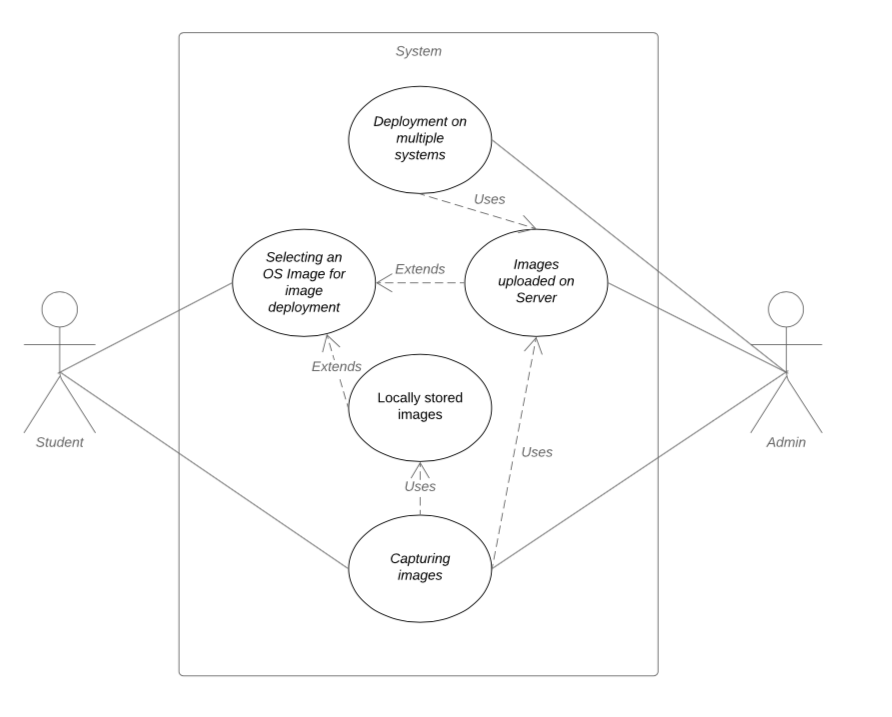
\includegraphics[width=\linewidth]{i1.png}
    \caption{Use Case diagram of the system}
    \label{fig:Use case}
    \small
    ( Student chooses the image to be deployed from the central server or local harddisk
    Administrator maintains the central repository of images and can deploy
    images to any of the clients remotely )
\end{figure}

\subsection{\usefont{T1}{phv}{b}{it}User requirements}
\begin{enumerate}
\item Automate without any manual intervention in installing OS having specific software.
\item In the lab, the requirement is to have different OS  /software or both for each lab session, i.e., there is a need for frequent imaging and also the same set of OS/software needed after some period.
\item Easy to set up and manage image capture and deployment ( admin point of view) system.
\item Keeping one of the storage partitions unaffected by imaging in a client machine, where the clients can store the files.
\item Both the client and the lab admin can capture and store images. The client may have installed and configured new software, he/she may want to use the same configured OS, the next time he/she comes to that lab, i.e., they have to have the ability to capture the OS image and then restore it whenever needed.
\item Give support for both Windows and Linux based distribution OS images.
\item Give support to heterogeneous environments of UEFI and BIOS firmware based clients.
\end{enumerate}
\subsection{\usefont{T1}{phv}{b}{it}System requirements}
\begin{enumerate}
\item Client needs to be PXE enabled. Other than this, no other setup is required on the client-side.
\item Network connectivity through LAN cable.
\item Availability of servers to set up DHCP, TFTP, and storage servers
\item Integrate the DHCP server required by this system to an existing DHCP server.
\end{enumerate}

% \begin{enumerate}
%     \item Student has to choose the image which he/she wants to deploy,
%         \begin{enumerate}
%             \item Has to choose the image which he/she wants to deploy from either the local harddisk or the central server
%             \item Can make certain changes to the OS and save it locally after capturing for further use
%         \end{enumerate}
%     \item Administrator
%         \begin{enumerate}
%             \item Maintains the central repository which has all the images
%             \item Can deploy images to any of the clients remotely
%         \end{enumerate}
% \end{enumerate}


\newpage

\section{\fontsize{16pt}{1em} \usefont{T1}{phv}{b}{}Methodology}
% Remote OS cloning and image deployment system orchestrates the image deployment through the collection of server interaction without any initial client software except for PXE enabled client, i.e., bare-metal client. 
Image cloning and deployment can be done in two ways, through network orchestrated image deployment on the bare-metal client or through software from inside the OS. It is difficult to clone the disk from inside the existing  OS of the client as \\
i)it requires the file system to be unmounted \\
ii) also, image deployment from within existing OS in the client will lead to inconsistencies. \\
iii) will not be able to control the image deployment remotely.\\
So the bare-metal client is used for imaging. The following problems arise when the image needs to  deployed on-the-fly to the bare-metal client:\\
i) How to boot the client from network \\
ii) How to deploy an image if no imaging software is present in the client \\
iii) How to deploy OS image to client from remote computer \\
Remote OS cloning and image deployment system orchestrates the image deployment through the collection of server interaction without any initial client software except for PXE enabled client, i.e., bare-metal client. The required software such as bootloader and the image deployment tool is loaded from network to memory through PXE booting.
\subsection{\usefont{T1}{phv}{b}{it} PXE Boot}
PXE ( Preboot Execution Environment) technology allows a client to boot from a network loaded operating system through support of PXE enabled servers. PXE technology is firmware that supports industry-standard Internet protocols, namely UDP/IP, DHCP and, TFTP. It is present in all Intel-based computers, but it needs to be PXE enabled and connected through LAN cable to a network containing PXE enabled servers. 
PXE enabled servers to refer to a set of servers that support PXE client specifically for PXE boot. It contains the following components summarised in fig 4.1 : 
\begin{enumerate}
 \item DHCP server: It assigns the IP address to LAN PXE client, gives the name of the boot file and location (IP address) of the TFTP server to access it in addition to normal DHCP servers which only assigns the IP address.
 \item  TFTP server: It stores boot files (bootloader and OS), which  PXE client downloads after IP assignment. TFTP is used be because it is easily implemented in the client's NIC firmware, resulting in standardized small-footprint PXE ROMs
 \item  Network Bootloader and OS: A Network bootloader to be able to boot a tiny network OS from the network ( Contains the image cloning and deployment tools). Both of them are present on the TFTP server.
 \end{enumerate}
 The PXE client network boots by connecting to a network and requests an IP address and the location of the bootloader. The DHCP server assigns an IP address and sends a boot file name along with the IP address of the TFTP server. The PXE client then retrieves the GRUB modules from the TFTP server and loads GRUB, the GRUB boots, into a tiny operating system located on the TFTP server.
 \begin{figure}[h!]
    \centering
    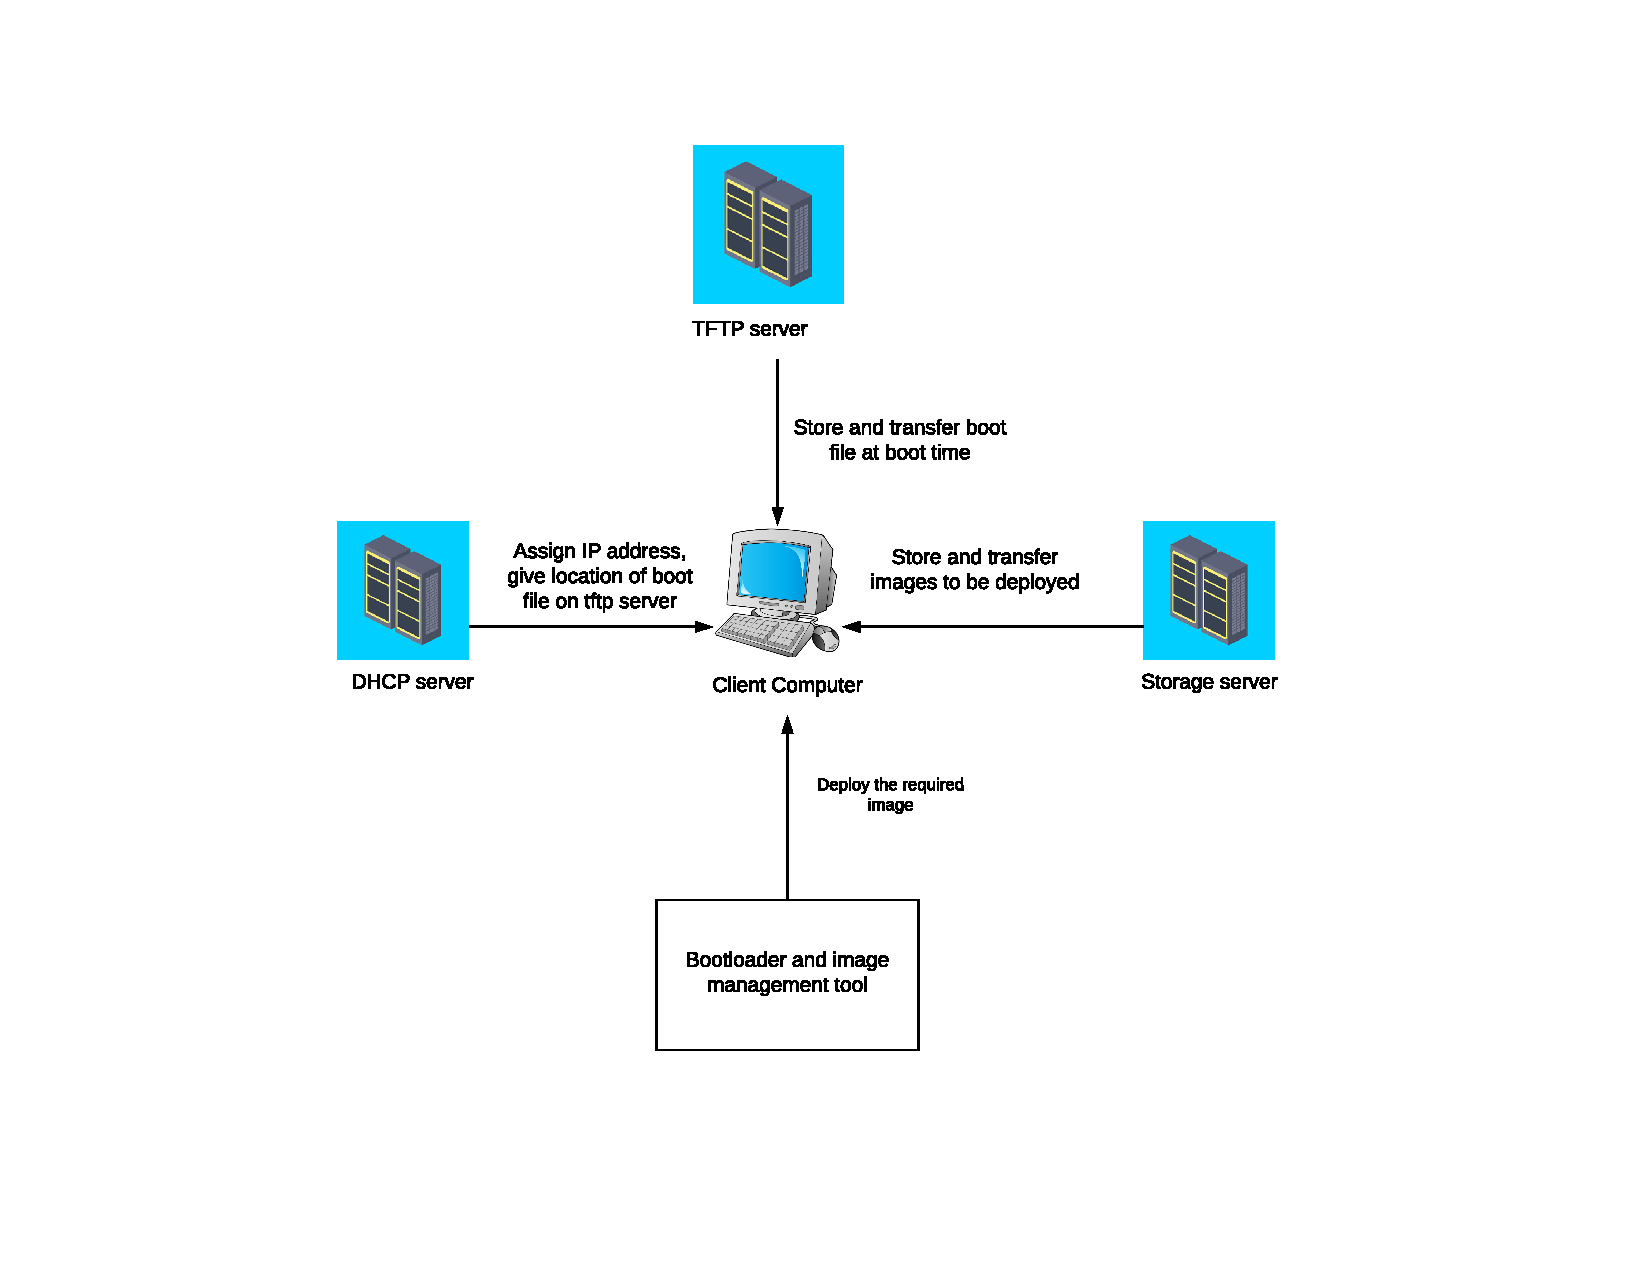
\includegraphics[width=\linewidth]{basicsysarch.pdf}
    \caption{Basic System Architecture}
    \label{sys_arch}
\end{figure}


% 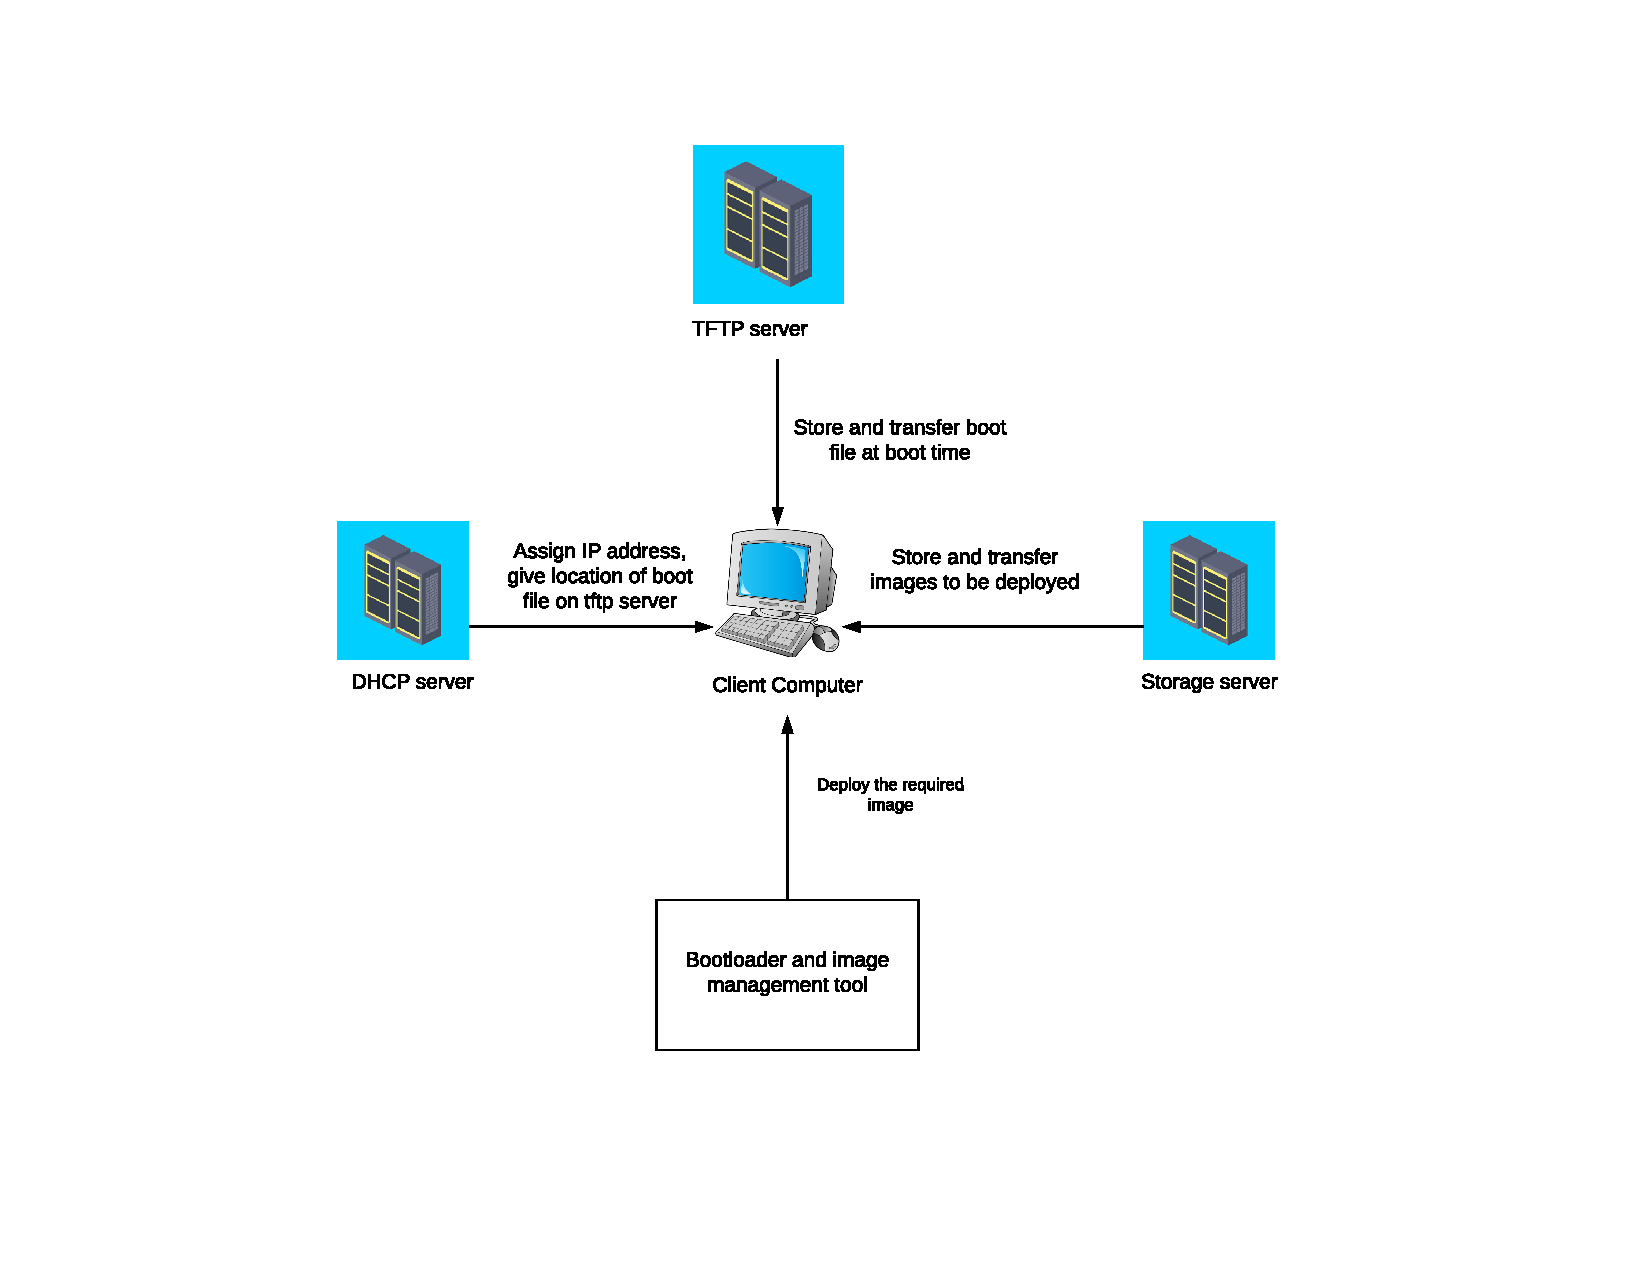
\includegraphics[page=1, trim = 18mm 80mm 18mm, clip, width=14.35cm]{basicsysarch.pdf}
% \captionof{figure}{Basic System Architecture} 
\subsection{\usefont{T1}{phv}{b}{it} Remote Image cloning and Deployment System}
  The network booted OS contains tools for cloning and imaging. A storage server is needed to store cloned images. It is used in the fast transfer of images from the server to the client during deployment and from client to server during cloning.
  The tiny operating system displays a menu ( if its not deployed by the admin ) of available images on the storage server, and when a choice is made by the client, that particular image is downloaded from the storage server and then deployed. Then the system reboots directly to the deployed image. A web interface is designed to handle all the operations at the admin side.
  The entire workflow is summarised in flowchart fig 4.2
  \newline
%\\
%  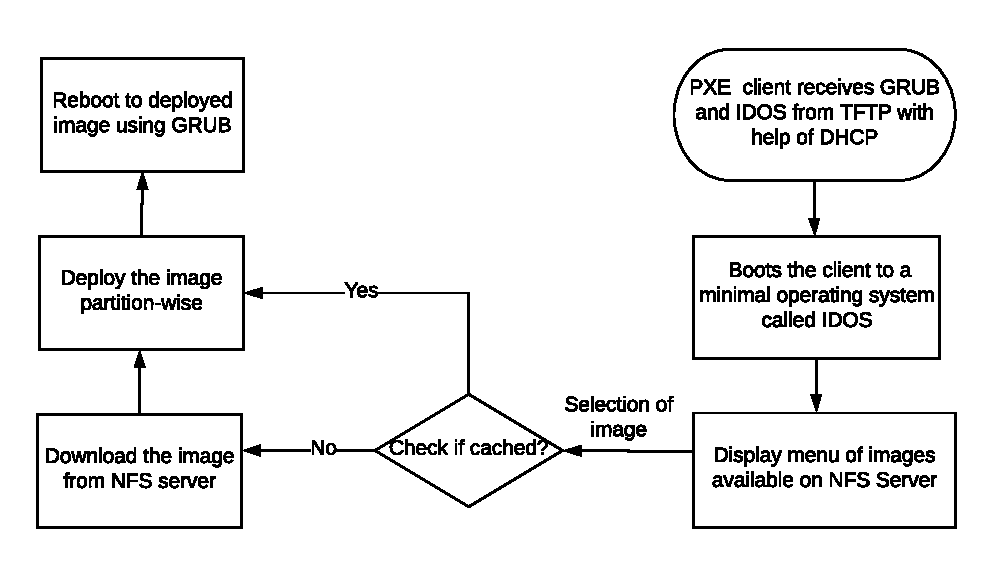
\includegraphics[page=1, trim = 18mm 80mm 18mm, clip, width=14.35cm]{Workflow.pdf}
%  \\
%  \\
%  \\
\subsection{\usefont{T1}{phv}{b}{it} Image cloning and deployment management}
Image cloning and deployment management are done using a web application. Through the web application, the user (admin/student) can perform tasks like cloning, image deployment to any of the listed clients present in the database. For e.g., the user chooses one of the clients, creates an image deployment task by selecting one of the available images in the storage server. The tasks created are stored in the database, and when the client is up, the client IDOS communicates with the web app to check if there is any task to be performed on it using suitable APIs. If there exists any task for it, IDOS performs the task on that client, and on successful completion of the task, the client signals task completion to the web server, after which the webserver removes the task from the database. If no assigned task exists, the client-driven image cloning/deployment is done. The flowchart fig \ref{fig:detailed design} summarizes the working of image deployment through a web application as well as client-driven deployment.
\subsection{\usefont{T1}{phv}{b}{it}Detailed Design methodology}
The previous section described the design of system architecture, which fulfills the basic requirements of the system. This section discusses how to include other desired requirements in the design of the project. This includes how to design an automated image deployment system using GRUB  and design the cache mechanism to lower the network traffic, hence improve the performance of the system.
\subsubsection{\usefont{T1}{phv}{b}{it}Booting from local HDD using Network GRUB  }
\paragraph{}
One of the objectives of the project is to boot the deployed image after deployment. After the image deployment, the IDOS reboots and again loads the GRUB. The network loaded GRUB must be able to boot from local HDD in addition to booting from the network. The main challenge is to locate the image deployed in the specific client by the network GRUB so that it can load the OS from the HDD.
\paragraph{}
To enable the above functionality, after IDOS deploys the image onto the HDD, a GRUB utility, which is termed as 'grub-mkconfig,' is used, which locates the kernel, initramfs files in the deployed image and generates the GRUB configuration file. This generated the GRUB config file of a specific client is stored in the TFTP server. So on the next boot, GRUB can fetch this client-specific config file and thereby able to boot from local HDD also. 
\subsubsection{\usefont{T1}{phv}{b}{it}Cache Mechanism}
\paragraph{}
As stated in section 2, an image is reused periodically.  Instead of downloading the same image every time, which leads to higher network traffic, the cache mechanism at the client-side would prevent re-downloading of the same image.
\begin{figure}[h!]
    \centering
    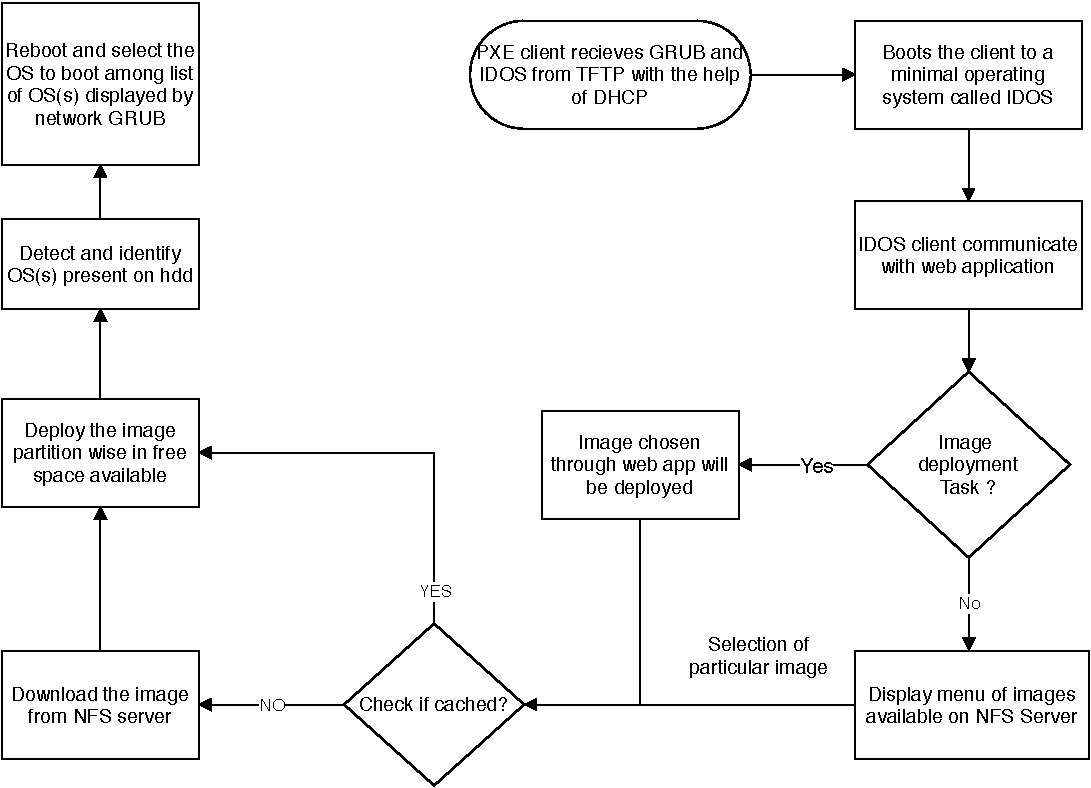
\includegraphics[width=\linewidth]{flowchart.pdf}
    \caption{Flowchart of remote OS image deployment }
    \label{fig:detailed design}
\end{figure}

\paragraph{}
A simple cache mechanism is developed where a portion of local HDD called hidden partition (usual, the end of the disk) is reserved for storing the compressed OS image as cache. Whenever a choice of image is made, the IDOS checks if the image is present in the cache. If the image is not present, it downloads the image from the NFS server into the cache ( if enough space is available, it is downloaded. If not, it does not download to the cache rather directly deploys to local HDD. This problem can be solved by adopting a suitable cache replacement mechanism ) and then deploys the image from the cache. If the image is already present in the cache, it deploys from the cache without downloading, thereby decreasing the network traffic. This workflow is summarised in fig \ref{fig:detailed design}.

\subsubsection{\usefont{T1}{phv}{b}{it} Supporting Image deployment on existing OS(s) system and Multi-booting}
In the earlier works, OS image deployment led to the erasing of existing OS(s) from the HDD as the deployment was overwriting the existing partitions. The feature to multi-boot the system after image deployment with existing OS(s) has two problems: \\ 
i) Disturbing the existing OS(es) during image deployment and \\
ii) Detect multiple Operating Systems existing on HDD and able to boot to them using a bootloader.

To not disturb existing OS(es) while image deployment, two solutions are possible:
i)one is to image to free space and \\
ii)Delete any partition or resize the partitions to free space.\\
Solution i) is more elegant than the other, and so was implemented. Please refer to this in section 5.5. This method is limited when there is no enough free space for imaging.

After OS image deployment, the bootloader needs to identify the deployed OS and also the existing OS(es). The bootloader present on HDD knows only about existing OS(es) and not deployed image. Also, it is difficult to locate the bootloader in HDD to communicate the new imaged OS. The use of grub-utilities and the network GRUB, to identify and load multi-boot OSes.





% \newpage
% \section{\fontsize{16pt}{1em} \usefont{T1}{phv}{b}{}Results and Analysis}


% \newpage
% \section{\fontsize{16pt}{1em} \usefont{T1}{phv}{b}{}Conclusion \& Future Work}
\newpage
\section{\fontsize{16pt}{1em} \usefont{T1}{phv}{b}{}Work Done}
In this semester we developed the proof of concept of the design through a prototype. We first implemented the PXE boot and then worked on remote cloning and image deployment system. The prototype consists of various components as discussed in the following subsections. It currently supports cloning and imaging in legacy BIOS computers and partially UEFI computers. 
\subsection{\usefont{T1}{phv}{b}{it} Setting up of Servers}
As discussed in section 3, to implement the PXE boot and storage server, we require DHCP, TFTP server and NFS server. It was setup as follows:
\begin{enumerate}
    \item TFTP server: 'tftpd-hpa' package is used to create the TFTP server. It is configured to share  “/tftpboot” directory with read and write access, from which the client can fetch the file from TFTP and also can put the file into TFTP server/ "/tftpboot" directory. The directory contains  GRUB core image and modules for different platforms (BIOS,  UEFI x86\_32, UEFI x86\_64 ), IDOS image. The TFTP server supplies the corresponding GRUB to the PXE client, as requested by the PXE client. The client then loads the bootloader and further downloads the IDOS image and boots to IDOS. TFTP server is containerized and deployed on Ubuntu 18.04.
    \item  NFS server: 'nfs-kernel-server' package is configured to share “/nfsroot” directory with mount options to all computers in the same network. The "/nfsroot" directory contains the cloned images, automated cloning and image deployment scripts, and the GRUB utilities. On boot of IDOS, IDOS mounts the NFS server, and then it executes the automated clone and image deployment script. NFS server is set up on Ubuntu-18.04. 
\end{enumerate}
\subsection{\usefont{T1}{phv}{b}{it} Network GRUB}
Network bootable GRUB is built from the source \cite{GRUB}. Blog \cite{PXEb} provides the information on building network bootable GRUB and how to PXE boot using this GRUB. GRUB utilities - 'grub-mkimage' and 'grub-mknetdir' are used to build core and network bootable GRUB modules, respectively. Currently, the GRUB-2.02 version is used for the project. Network GRUB consists of a core image and various modules which are placed in the TFTP server. PXE client first loads the core image, and control is handed over to core GRUB, which subsequently downloads the required modules. The modules are loaded from the TFTP server as and when that functionality is required. Suppose to read the HDD, and the GRUB core downloads the part\_msdos and ext4/ntfs modules. The GRUB bootloader is platform-specific, i.e., needs different GRUB builds for different firmware clients. The i386-pc, x86\_32-efi and x86\_64-efi, GRUB builds correspond to BIOS,  UEFI x86\_32 and UEFI x86\_64 PXE clients. Depending upon the type of client, the DHCP sends the location of these builds. Once GRUB is loaded, it boots to either network loaded IDOS or from local HDD depending on the selection by the user in the GRUB menu, as shown in Fig \ref{grub}. 
\begin{figure}[h!]
    \centering
    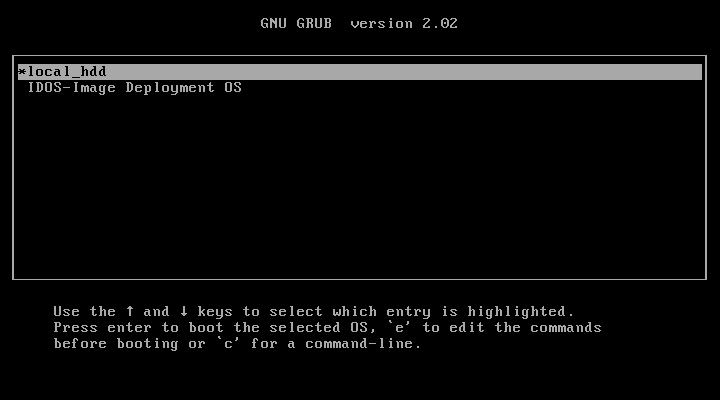
\includegraphics[width=\linewidth]{grub.png}
    \caption{Network GRUB Menu}
    \label{grub}
\end{figure}

Booting from HDD using GRUB is achieved by generating GRUB configuration (grub.cfg) after the image is deployed by using the GRUB utility termed as 'grub-mkconfig'. The 'grub-mkconfig' scans the HDD for OS(s) and generates a 'grub.cfg' which contains the location of Linux kernels and initramfs in case of Linux and chain bootloader in case of Windows. Currently, this project supports the only detection of Linux based OS through 'grub-mkconfig' and hence supports only Linux based OS booting from local HDD.
\subsection{\usefont{T1}{phv}{b}{it} IDOS (Image Deployment OS) }
IDOS is a Linux-kernel 5.1 based operating system developed from source using a tool called  Buildroot\cite{buildroot}. The tool helps in building the Linux kernel from scratch with only the required packages/tools such as 'mke2fs', parted as discussed further in this subsection. Partclone tool which helps in cloning and imaging sparse images is integrated into Buildroot as an external package. To integrate the Partclone package in Buildroot, additional config files are added to Buildroot, which assists the Buildroot in building the package from the source and integrating it to the root filesystem of IDOS.

\begin{figure}[h!]
    \centering
    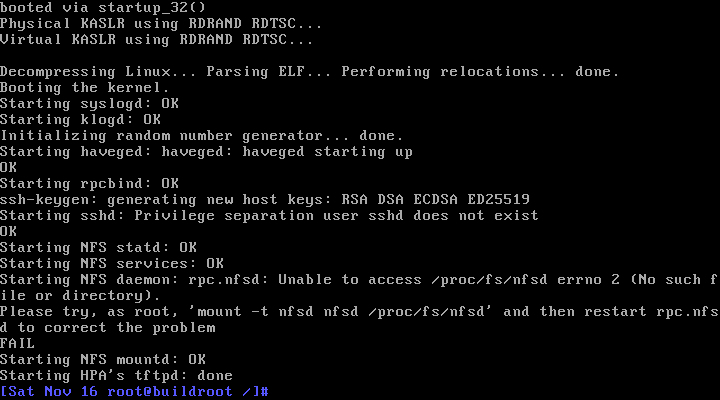
\includegraphics[width=\linewidth]{booting_IDOS.png}
    \caption{IDOS booting}
    \label{b_IDOS}
\end{figure}
\begin{figure}[h!]
    \centering
    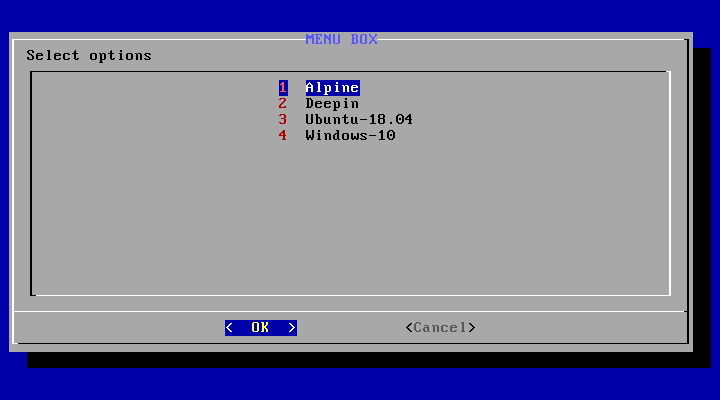
\includegraphics[width=\linewidth]{menu.png}
    \caption{Menu displaying various OS images present at the NFS server}
    \label{Menu}
\end{figure}
\begin{figure}[h!]
    \centering
    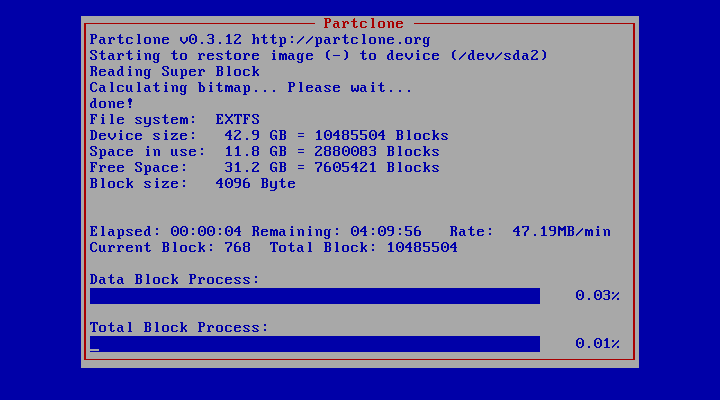
\includegraphics[width=\linewidth]{partclone.png}
    \caption{Sparse Image deployment by Partclone tool}
    \label{partclone}
\end{figure}

IDOS is loaded by the GRUB from the TFTP server in bzImage format and boots, as shown in Fig \ref{b_IDOS} . The IDOS displays the menu of available images from the mounted NFS-server using a dialog tool, as shown in Fig \ref{Menu}. Depending upon the selection of image, that image is downloaded in compressed form by the client machine using copy (cp command) if it is already not cached. It then uncompresses the image using gzip and then deploys it on to local HDD using Partclone. Before displaying the menu items, the IDOS checks if there exists a hidden partition. If not, a partition is created at the end of the HDD by reserving a space of size equal to 20\% of the total size of HDD using the 'parted' tool. It then formats using the 'mke2fs' tool and mounts the partition and copies the partition table to the NFS server. Then it displays the menu entries. Before downloading the chosen image, it checks whether the image is locally present by comparing the md5sum of images present in the hidden partition and that of the selected image in the NFS server. If locally present, it does not download the image again. Instead, it deploys the local image present to HDD using the Partclone tool, as shown in Fig \ref{partclone}.

Logging for each client is done and is stored on the NFS server. Logs contain the status of image deployment and client machine hardware information. The above-automated deployment is possible with a collection of scripts located at the NFS server, which uses necessary tools and commands. These scripts are run as part of the initialization process of IDOS.

\subsection{\usefont{T1}{phv}{b}{it} Experimental Setup}
DHCP and TFTP server is set up on one computer, and the NFS server is set up on the second computer. All the servers are set up on Ubuntu-18.04 OS. Along with the servers, three client computers were connected to Cat V network switch through cat 5e and cat 6 ethernet cables to form a LAN. LAN setup was common to both client setups. Clients are used as bare metal clients, i.e., no initial software installation is needed in both the client setup.
Two types of clients setup were done to test the proof of concept :

i) Cloning and Imaging in VM clients: One VM client per host of required configuration (memory, HDD, processor, network boot option) is spawned on three host machines. The VM is connected to the LAN interface of the host through a bridge adapter. Bridge adapter allows VMs to communicate with the above  LAN setup in the same way as the host computer. This was useful for development as well as testing the prototype in the initial phase.

ii) Computer clients: Computers are made PXE-enabled, and network boot option is set as the first boot option. The setup included both BIOS and UEFI computer clients. Three computer clients were used for this purpose.

\subsection{\usefont{T1}{phv}{b}{it} Supporting image deployment on existing OS(s)}
As mentioned in section 4.4.3, imaging is done on free space. Firstly, 
mber of partitions are created on HDD, and currently, this work supports 'MSDOS' and 'GPT' \cite{GPT} partition tables. In the 'MSDOS' partition table present in MBR \cite{MBR}, the number of 'primary' partitions are tracked so that it does not go above three partitions and if more partitions are required, they are made as 'logical' partitions in 'extended' partition. Most BIOS legacy systems use the 'MSDOS' partition table, and UEFI systems use the 'GPT' partition table. So, now the image deployment system supports both BIOS \cite{BIOS} and the UEFI \cite{UEFI} systems completely. After the creation of partitions, the OS image is deployed partition wise.
\subsection{\usefont{T1}{phv}{b}{it} Multi-booting with other existing OS(s)}
Grub utility called 'grub-mkconfig' detects and identifies different OSs for GRUB in a multi-boot system. The grub-mkconfig tool is integrated into IDOS. The grub-mkconfig, in turn, uses two main tools: \\
i) os-prober \cite{osprober} : This tool detects OSs and partitions where they are present on HDD. It uses the linux-boot-prober tool to generate boot parameters for  Linux kernel. For other OSs, the os-prober finds the boot parameters through os-probes, e.g., Windows, MAC OS, etc. This tool needed to be customized and other dependency packages needed to be included in IDOS.\\
ii) linux-boot-prober: This tool used to generate boot parameters for different Linux distributions using 'linux-boot-probes'. This tool is used by os-prober and, in turn, by grub-mkconfig.
The tools: grub-mkconfig, os-prober, linux-boot-prober are integrated into IDOS using root filesystem overlay (rootfs\_overlay).
After the image deployment, the grub-mkconfig tool is to generate the GRUB config file for that specific client and stored in the TFTP server. On the next boot, the client loads this GRUB config from the TFTP server and displays the list of OSs present in the multi-boot system.
\subsection{\usefont{T1}{phv}{b}{it}Web based Image deployment management}
A web application was built using the Django framework to facilitate the management of image deployment processes. Django is a Python-based free and open-source web framework, which follows the model-template-view architectural pattern. SQLite database is used for storage. SQLite is a relational database management system contained in a C library. Currently, two functionalities are integrated with this web application.
\begin{enumerate}
     \item   Client Registration: Each client has to be registered in the web application. Whenever a client connects to the server and boots, it sends a request to the webserver along with the details such as its name and MAC address. The web application will automatically register this client if the client is not already registered. The details of this client will be stored in the database.
    
    \item Image deployment: The web application displays all clients who are registered. The administrator has the ability to choose any client and deploy an OS image to this client. The list of available OS images is stored in the database. The user will choose one of these images. A Task will be created and stored in the database representing the deployment of the image on a particular client. When the client boots, it sends a request asking for any pending tasks. This request is then responded with the previously created task.
\end{enumerate}



\subsection{\usefont{T1}{phv}{b}{it} Miscellaneous}
Following miscellaneous items were done:
\begin{enumerate}
    \item Reproducible builds and optimizing the size of IDOS: IDOS is a Linux distribution built using the Buildroot tool. Only the required packages are included to optimize the size of IDOS. The necessary config files, rootfs\_overlay, external package config (partclone) of Buildroot (see Buildroot Documentation \cite{buildrootdoc}), are saved, versioned, and built-in container for reproducible builds. This process makes in helping automate the builds of IDOS in the future.
    \item Resolving errors in shell scripts and structuring of scripts: Most of the project's functionalities are implemented in shell scripting, which is interpreted language having no error handling. Many errors were rectified by re-structuring a single script into many scripts, each having basic functionality. Cleaner code with functions is implemented.
    \item Resolving the need to build IDOS specific to a network and increasing ability to package: During initial works, the TFTP server, NFS server IP and parameters to mount were included in the ramfs of the kernel. For different networks, the IDOS needed to be rebuilt again. This was solved passed certain environment variables such as TFTP server IP, NFS server IP, Webserver IP, etc. to IDOS kernel at boot time as boot parameters in the GRUB config file. This makes IDOS independent of the network, and to deploy the system in different network only the GRUB config needs to be updated accordingly.
\end{enumerate}
% - buildroot
% - builds
% - scripts errors
% - IDOS independency - auto,man, VM, LAN 
 \newpage
\section{\fontsize{16pt}{1em} \usefont{T1}{phv}{b}{}Results and Analysis}
We did an analysis of two cloning image utilities through our prototype, which is data duplicator (dd) and Partclone on their cloning and imaging capabilities w.r.t space and time. The aim of the analysis is to show the superiority of Partclone over dd and also the advantage of implementing a cache mechanism to reduce network traffic.

\subsection{\usefont{T1}{phv}{b}{it} Comparing the sizes of cloned HDD images}

The size of the cloned image from each utility after compression is compared in Table \ref{images} for different OSs. Cloning is done on four different OSs, including Linux based and Windows OS. 

The OSs cloned are sparse images as the used disk is smaller than the actual size of the disk cloned. Partclone clones and images it as a sparse image, whereas dd doesn't support sparse image cloning and imaging. From, the table it can be seen that the Partclone efficiently clone only the sparse image and compresses it using gzip, which is much smaller in size compared to cloned image using dd.


\begin{table}[H]

\label{tab:title} 
\begin{center}
\begin{tabular}{|c|c|c|l|l|}

\hline
\begin{tabular}[c]{@{}c@{}}Image \\ Name\end{tabular} & \begin{tabular}[c]{@{}c@{}}Total size\\  of\\  image (GB)\end{tabular} & \begin{tabular}[c]{@{}c@{}}Sparse image \\ size (GB)\end{tabular} & \begin{tabular}[c]{@{}l@{}}Compressed\\  Partclone image \\ size (GB)\end{tabular} & \begin{tabular}[c]{@{}l@{}}Compressed \\ dd image (GB)\end{tabular} \\ \hline
Alpine                                               & 5.57                                                                   & 3.60                                                               & 0.76                                                                              & 1.74                                                                \\ \hline
Ubuntu 18.04                                          & 45.00                                                                     & 4.95                                                              & 1.66                                                                               & 6.84                                                                \\ \hline
Deepin                                                & 42.80                                                                   & 11.80                                                              & 2.50                                                                                & 2.80                                                                 \\ \hline
Windows                                               & 53.70                                                                   & 16.50                                                              & 6.60                                                                                & 8.10                                                                 \\ \hline
\end{tabular}
\caption {Comparison of sizes of cloned images using Data Duplicator ( dd ) and Partclone} 
\label{images}
\end{center}
\end{table}
\subsection{\usefont{T1}{phv}{b}{it} Analysis on Image deployment time }
Similar to the above analysis w.r.t cloning, analysis on single unicast image deployment at a time using different tools - Partclone and dd are conducted w.r.t time taken. Besides, analysis of concurrent imaging, i.e., time taken in image deployment in five computers concurrently (using Partclone) is studied, and analysis on developed cached image deployment (using Partclone) is done.

From Table \ref{imaging}, single unicast Partclone image deployment from the NFS server takes the least time compared to image deployment through dd and also better than cached image deployment, i.e., from local HDD using Partclone. Partclone does better than dd because smaller cloned image size can be transferred faster through the network than the cloned images of dd and also due to sparse image writing, i.e., write data only to used blocks and just syncs the unused blocks. The dd write even the unused blocks while imaging deployment. Cached image deployment is slower than single unicast image deployment using Partclone because the HDD I/O speed lesser than the network transfer speed. 

In concurrent image deployment, the same image is being downloaded by the different clients from the same NFS server, and these many unicast downloads lead to bottleneck at network cable from the NFS server to the switch. Thereby decreasing the rate of image transfer due to higher network traffic and hence increases the deployment time. But once the image is cached in the concurrently requesting clients, the clients no longer download the image from the NFS server. Instead, it deploys from the local HDD. Hence, caching reduces the network traffic and therefore reduces the time taken for image deployment. The caching reduces the image deployment drastically when compared to concurrent image deployment once caching is done. The network traffic problem is still not solved in concurrent non-cache image deployment, which happens when the cached image is not available at clients.  
\begin{table}[H] 

\begin{tabular}{|c|c|c|l|l|l|l|}
\hline
Image Name   & \begin{tabular}[c]{@{}c@{}}Sparse \\ Image \\ size (GB)\end{tabular} & \begin{tabular}[c]{@{}c@{}}Partclone \\ restore in \\ VM (s)\end{tabular} & \begin{tabular}[c]{@{}l@{}}Partclone \\ restore in\\ computer \\ (s)\end{tabular} & \begin{tabular}[c]{@{}l@{}}dd restore\\  in\\  computer \\ (s)\end{tabular} & \begin{tabular}[c]{@{}l@{}}Concurrent \\Image \\ deployment \\ (s)\end{tabular} & \begin{tabular}[c]{@{}l@{}}Cached\\  image \\ deployment \\ (s)\end{tabular} \\ \hline
Alpine      & 3.60                                                                  & 140                                                                       & 130                                                                               & 166                                                                         & 360                                                                              & 157                                                                          \\ \hline
Ubuntu 18.04 & 4.95                                                                 & 250                                                                       & 200                                                                               & 756                                                                         & 450                                                                              & 297                                                                          \\ \hline
Deepin       & 11.80                                                                 & 800                                                                       & 415                                                                               & 600                                                                         & 1200                                                                             & 500                                                                          \\ \hline
Windows      & 16.50                                                                 & 1050                                                                      & 700                                                                               & 886                                                                         & 1800                                                                             & 825                                                                          \\ \hline
\end{tabular}
\caption {Comparison of time taken in deploying the images using different methods} 
\label{imaging}
\end{table}
\subsection{\usefont{T1}{phv}{b}{it} Supporting Image deployment on existing OS(s) system and Multi-booting }
As discussed in section 4.4.3, 5.5, 5.6, support for Image deployment on existing OS(s) system and Multi-booting feature is included. The feature is tested by imaging OS on client having already one or more OSs.

Here, as shown in fig. \ref{before_image}, two OSs exist - Windows NT 6 and Ubuntu-18.04 on the client before OS imaging. Then Deepin OS image is deployed and rebooted. The GRUB now shows and can load three OSs, i.e., Windows NT 6, Ubuntu-18.04, and Deepin, as shown in fig. \ref{after_image}.
\begin{figure}[h!]
    \centering
    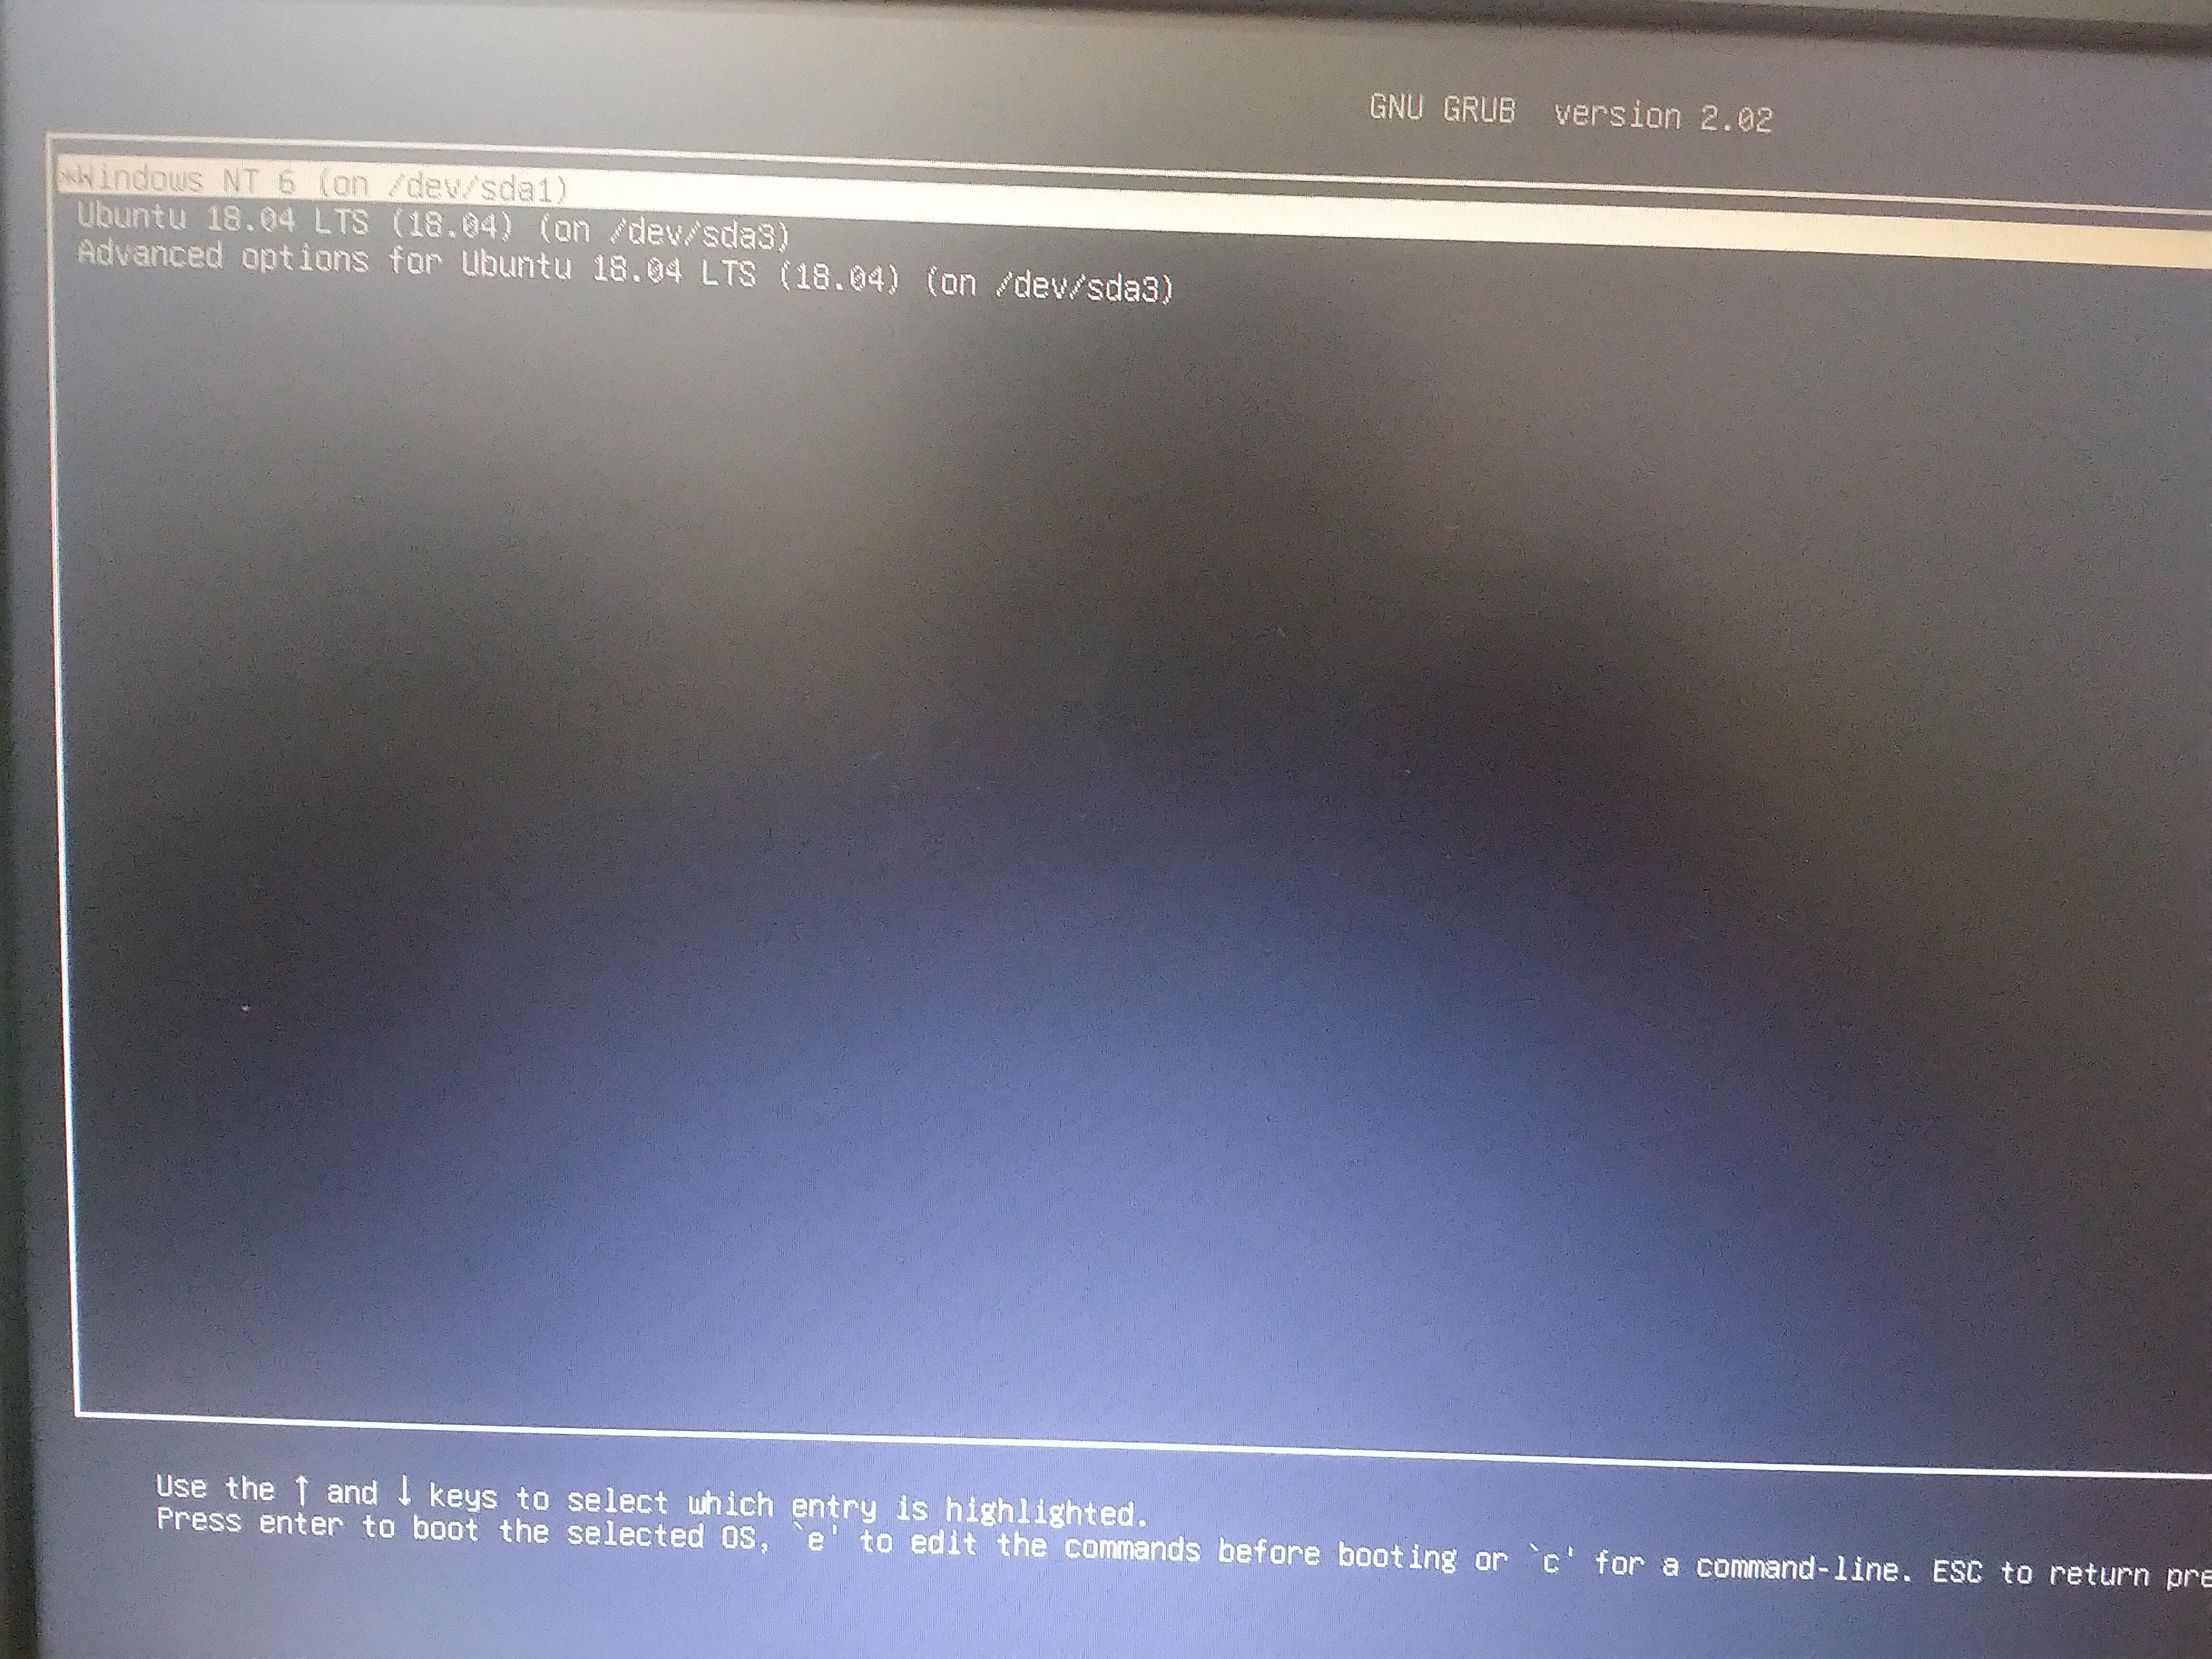
\includegraphics[width=\linewidth]{before_deploy.jpg}
    \caption{Existing OSs before image deployment}
    \label{before_image}
\end{figure}
\begin{figure}[h!]
    \centering
    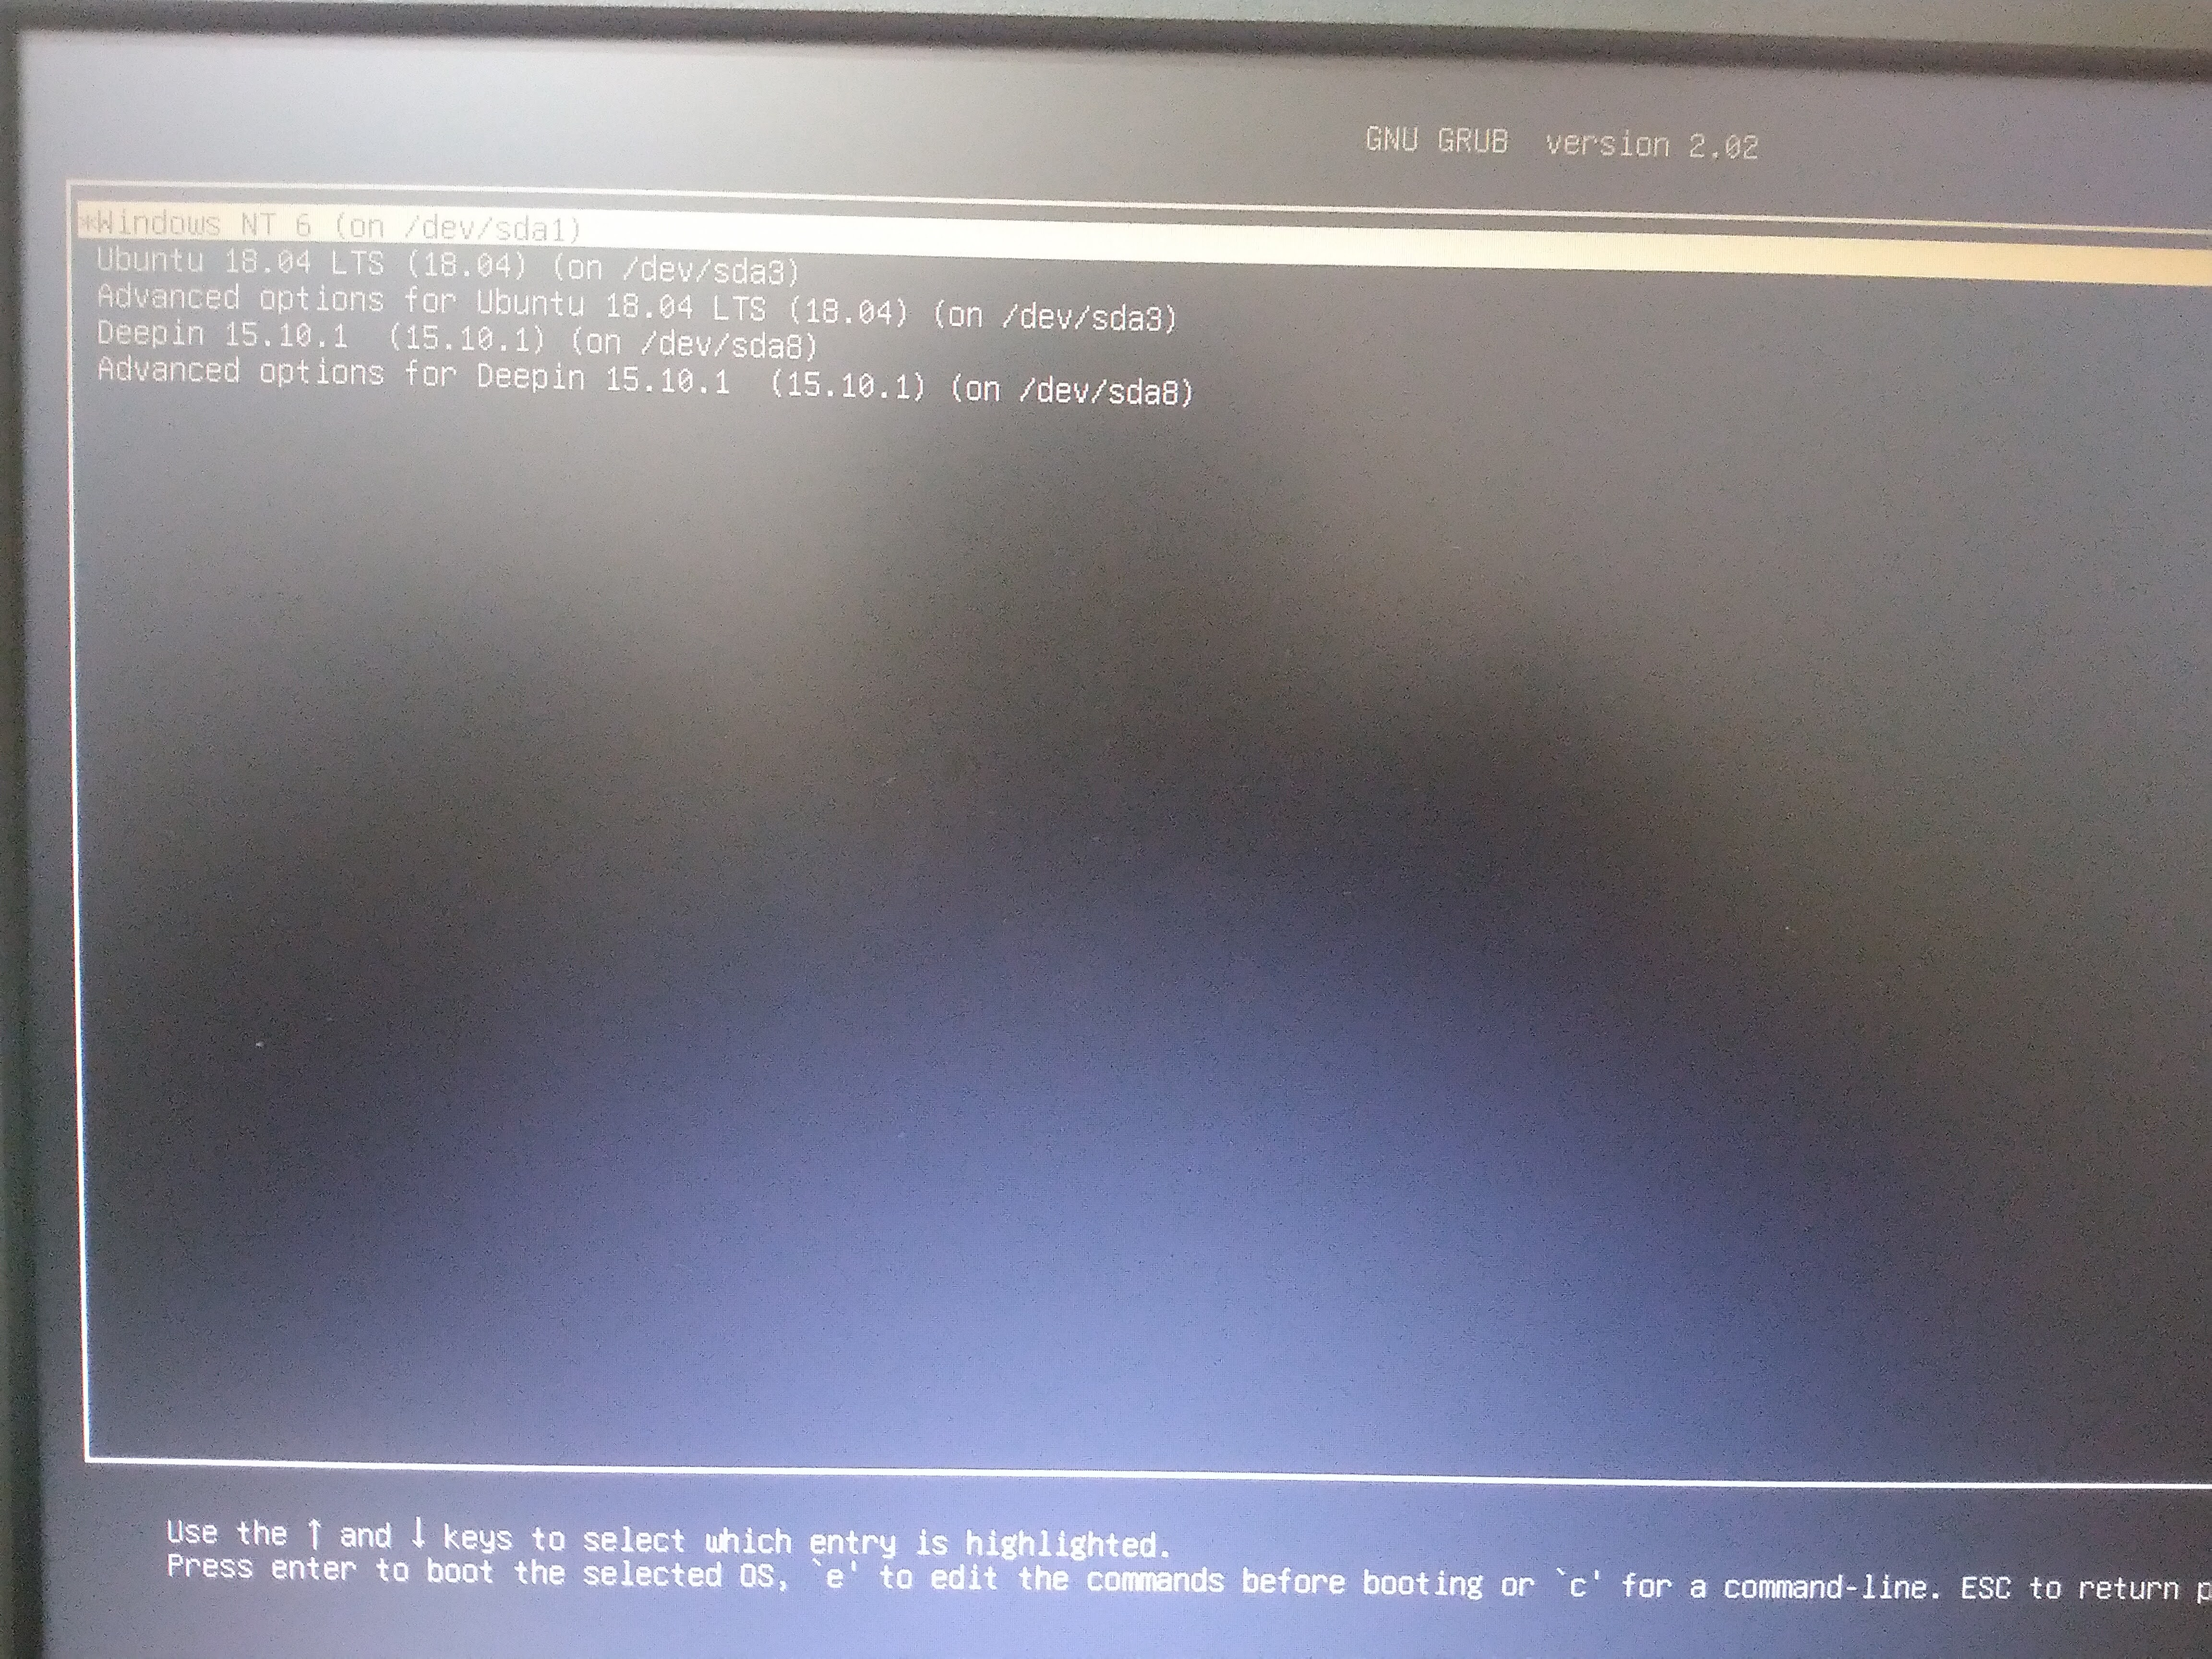
\includegraphics[width=\linewidth]{after_deploy.jpg}
    \caption{Multi-boot with existing OSs and deployed Deepin OS image}
    \label{after_image}
\end{figure}
% screenshot of existing oS
% screenshot after image deployment to show multi-boot support
\newpage
\subsection{\usefont{T1}{phv}{b}{it} Web application for image deployment management }
Various screenshots of Web UI are shown to demonstrate the features of the web application. Fig. \ref{home_page} shows the home page of the web app ROSIM (Remote OS Image Management), it contains login for users (admin/student), Clients, About tab at the top. All the registered clients are displayed with their MAC address at the Client web page shown in fig. \ref{reg_clients}. If one of the clients is chosen for the task, it redirected to another page having drop-down button consisting of all the available images is provided shown in fig. \ref{task_image_deploy}. After choosing the relevant image, the administrator can deploy the image to a particular client.
\begin{figure}[h!]
    \centering
    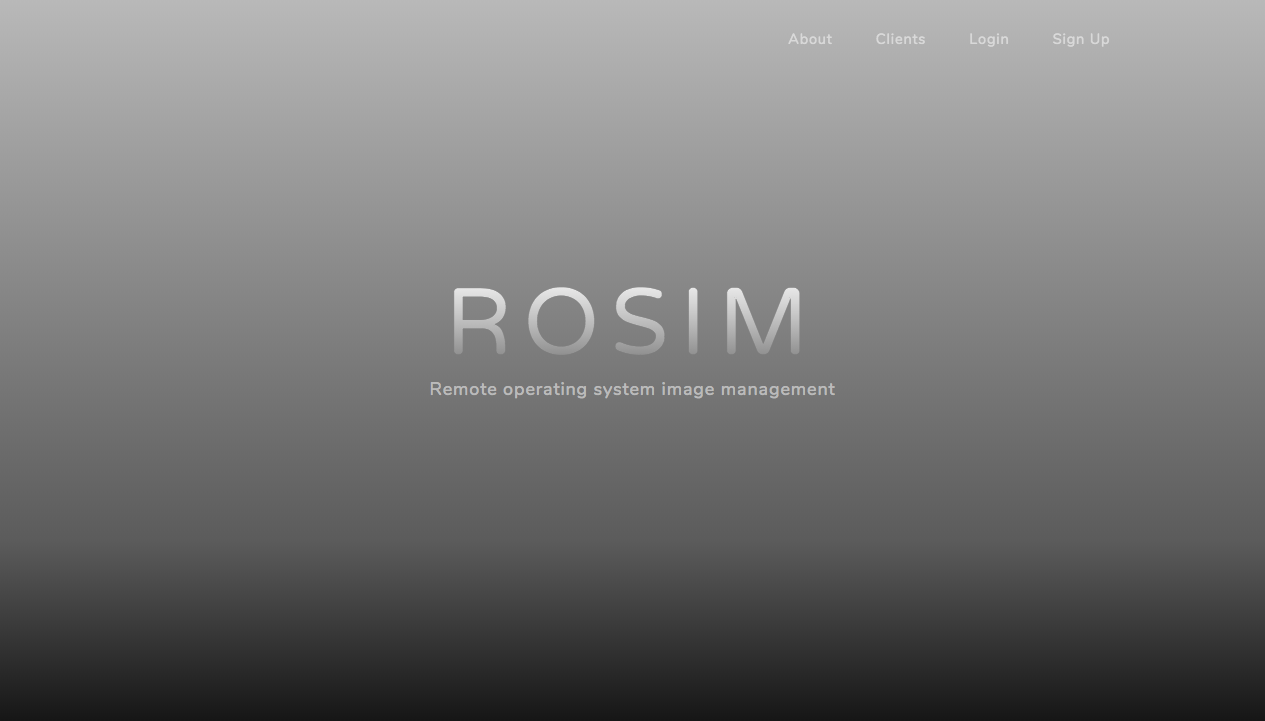
\includegraphics[width=\linewidth]{webapp1.png}
    \caption{Home page}
    \label{home_page}
\end{figure}
\begin{figure}[h!]
    \centering
    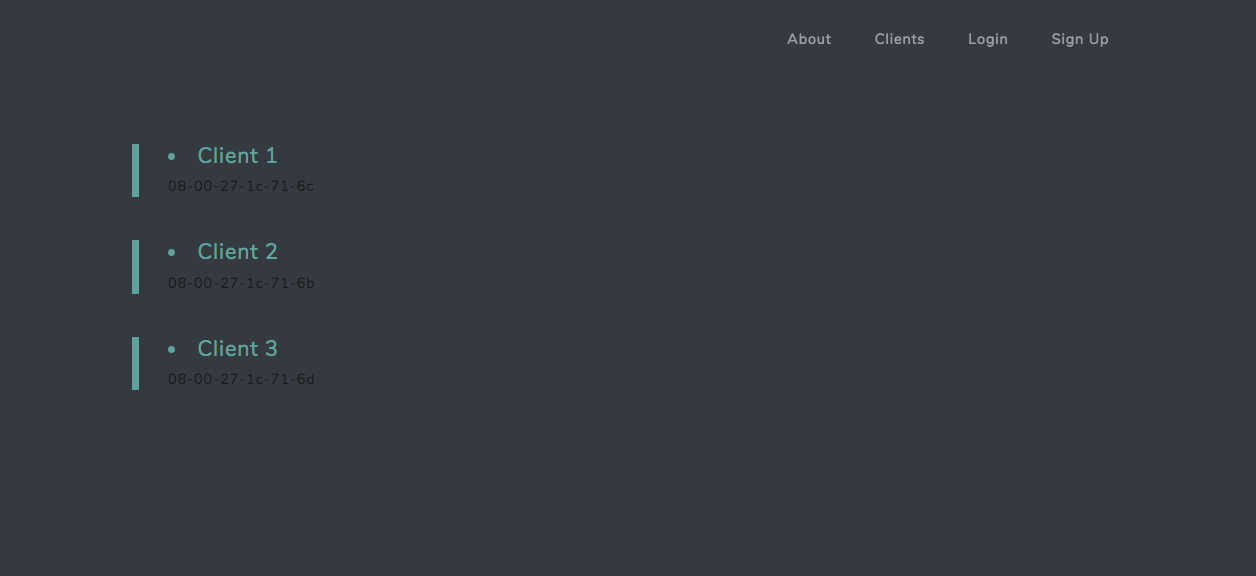
\includegraphics[width=\linewidth]{webapp2.png}
    \caption{List of registered clients}
    \label{reg_clients}
\end{figure}
.
\newpage
\begin{figure}[H]
    \centering
    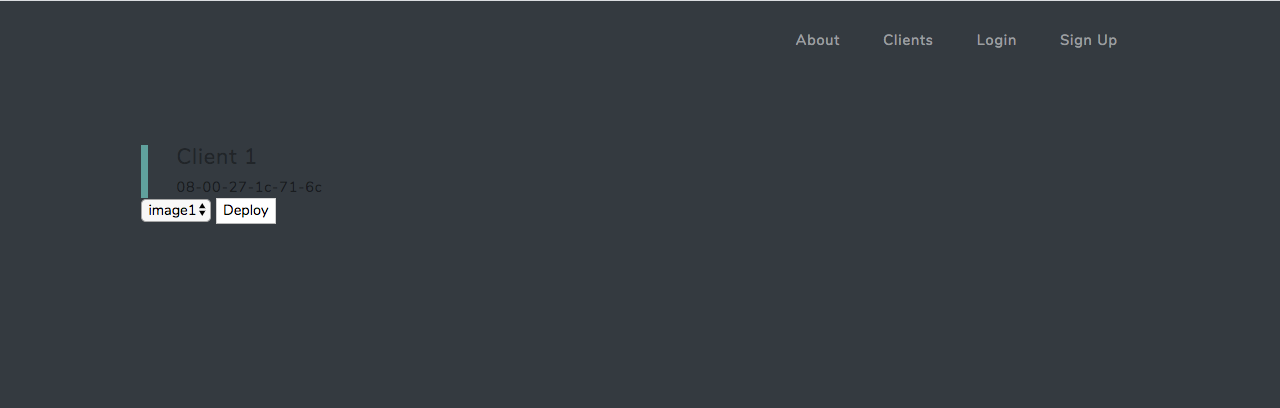
\includegraphics[width=0.9\linewidth]{webapp3.png}
    \caption{Choosing an image which has to be deployed}
    \label{task_image_deploy}
\end{figure}

%home page
%client registration
%image deployment
\newpage
\section{\fontsize{16pt}{1em} \usefont{T1}{phv}{b}{}Conclusions and Future work}
 The designed architecture, i.e., PXE boot, remote OS cloning, and image deployment and web base image cloning and deployment management, are implemented in the form of a prototype. Currently, this project supports re The designed architecture, i.e., PXE boot, remote OS cloning, and image deployment and web base image cloning and deployment management, are implemented in the form of a prototype. Currently, this project supports remote OS client-driven and web-based image deployment to VM or bare metal clients using Partclone, which are connected through a LAN network. The cloned OS images are deployed on the r

mote OS client-driven and web-based image deployment to VM or bare metal clients using Partclone, which are connected through a LAN network. The cloned OS images are deployed on the remote machines as expected, and the clients can multi-boot into any one of the OSs. The cache mechanism is partially implemented. The image deployment system supports UEFI firmware clients completely. The following work has to be carried out in the future.
\begin{enumerate}
    \item Implement suitable cache replacement policy  
    \item Improve Web UI and add features such as cloning, group image deployment.
    % \item Currently, only BIOS systems are supported. Support for UEFI systems must also be developed
    \item Instead of unicast image deployment in concurrent imaging, multicast imaging performs better and is more efficient as it transfers only one image through the network to multiple clients, thereby reducing the network traffic.
    % \item Support partition wise OS imaging and booting must be included
    \item Proper Scaling and testing measures must be undertaken
\end{enumerate}


%create BibTex files for references
\newpage
% \section*{\fontsize{16pt}{1em} \usefont{T1}{phv}{b}{}References}
\bibliography{MP.bib}
% \begin{enumerate}
%     \item Josh A. Meek, Michael K. Bradshaw et al. Web-Based Computer Lab Imaging with Grimiore. In Proceedings of the 37th annual ACM SIGUCCS fall conference: communication and collaboration ( 2009 ) doi: 10.1145/1629501.1629507
%     \item Li linhui, Zhang Ke, Zhang Fang et al. Network Center's Highly-Efficient Management Solutions based on Intel PXE-based Remote Cloning System.
%     In 3rd International Conference on Advanced Computer Control (ICACC 2011)
%     \newline
%     doi: 10.1109/ICACC.2011.6016442
%     \item \href{https://fogproject.org/}{FOG Project} - A free open-source network computer cloning and management solution
%     \newline
%     \url{https://fogproject.org/}
    
%     \item Wikipage of FOG project
%     \newline
%     \url{https://wiki.fogproject.org/}
%     \item PXE - Preboot execution environment
%     \newline
%     \url{https://en.wikipedia.org/wiki/Preboot_Execution_Environment}
%     \item Partclone - Partition clone and restore tool
%     \newline
%     \url{https://www.partclone.org/}
%     \item Partimage - Open source disk backup software
%     \newline
%     \url{https://www.partimage.org/}
%     \item IPXE - Open source network boot firmware
%     \newline
%     \url{https://ipxe.org/}

% \end{enumerate}
\newpage
\section{\fontsize{16pt}{1em} \usefont{T1}{phv}{b}{}Glossary}
\begin{enumerate}
       \item BIOS: BIOS (an acronym for Basic Input/Output System and also known as the System BIOS, ROM BIOS, or PC BIOS) is the firmware used to perform hardware initialization during the booting process (power-on startup), and to provide runtime services for operating systems and programs.
    \item dd: dd is a command-line utility for Unix and Unix-like operating systems; the primary purpose is to clone/ create a backup and restore/write the hard disk. This tool even
    \item DHCP: The Dynamic Host Configuration Protocol (DHCP) is a network management protocol used on UDP/IP networks whereby a DHCP server dynamically assigns an IP address and other network configuration parameters to each device on a network so they can communicate with other IP networks.
    \item HDD: It refers to a hard disk drive.
    \item IDOS: Image Deployment operating System (IDOS), is a customized Linux based OS developed from Buildroot for this project. It contains tools for image deployment.
  
     \item MBR: A master boot record (MBR) is a special type of boot sector at the very beginning of partitioned computer. The MBR holds the information on how the logical partitions, containing file systems, are organized on that medium.
    \item NFS: Network File System (NFS) is a distributed file system protocol, allowing a user on a client computer to access files over a computer network, much like local storage is accessed.
    \item PXE: The Preboot eXecution Environment (PXE) specification describes a standardized client-server environment that boots a software assembly, retrieved from a network, on PXE-enabled clients. Here, PXE-enabled client is used to network boot to IDOS on the bare metal client.
    \item TFTP: Trivial File Transfer Protocol (TFTP), a simple UDP based file transfer protocol that is compatible with PXE client.
    \item GRUB: GNU GRUB (short for GNU GRand Unified Bootloader, commonly referred to as GRUB) is a boot loader package from the GNU Project. 
    \item UEFI: The Unified Extensible Firmware Interface (UEFI) is a specification that defines a software interface between an operating system and platform firmware. Its function is similar BIOS, but UEFI is the new version of firmware, which supports more number of primary partitions, unlike  BIOS, which has MBR and supports only four primary partitions.
    \item Sparse Image: In this context, it refers to a disk image containing a sufficient amount of free space compared to the used space of the disk.
    \item Multi-boot: Multi-booting is the act of installing multiple operating systems on a computer, and being able to choose which one to boot. The term dual-booting refers to the common configuration of specifically two operating systems. Multi-booting may require a custom boot loader. 
\end{enumerate}
\newpage
\section{\fontsize{16pt}{1em} \usefont{T1}{phv}{b}{}Timeline}
 \begin{figure}[h!]
    \centering
    % 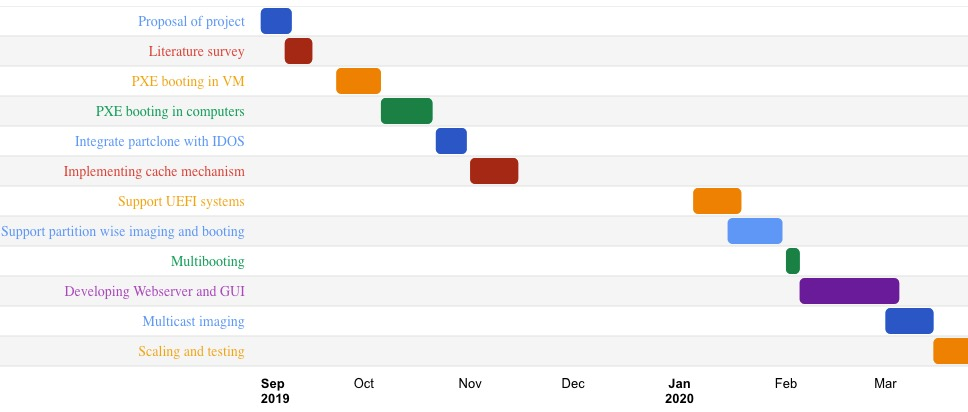
\includegraphics[width=\linewidth]{timeline.jpeg}
    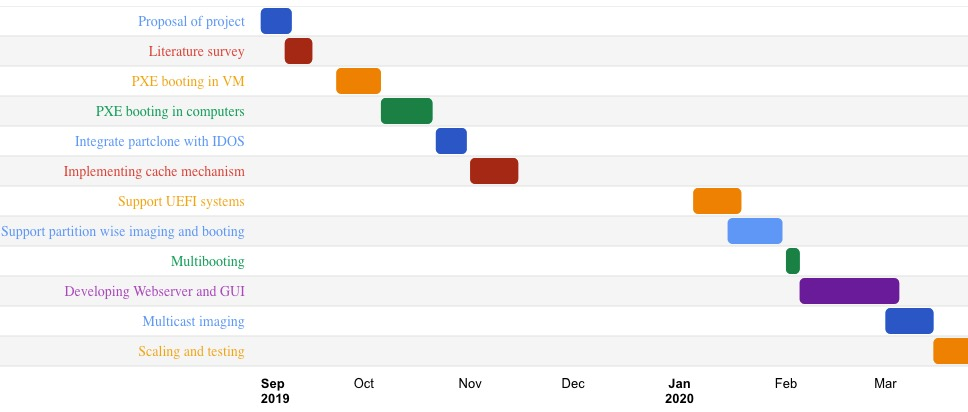
\includegraphics[height=4in, width=7in, angle=-90]{timeline.jpeg}
    \caption{Timeline of work}
    \label{timeline}
\end{figure}

\end{document}
